
\section{The INPUT files}
\label{inputfiles}

\begin{figure}[ht]
\begin{center}
\centerline{\psfig{file=dlpoly.files.ps,height=12cm}}
\caption{\D{}  input and output files}. 
\end{center}
Input files appear on the left and output files on the right. Files
marked with an asterisk are non-mandatory. File CFGMIN (not shown)
appears as an output file if the user selects the programmed
minimisation option (see \ref{minimisation}).
\end{figure}

In normal use \D{} requires six input files named CONTROL, CONFIG, FIELD, TABLE,
TABEAM and REVOLD. The first three files are mandatory, while files TABLE and
TABEAM (TAB/EAM in the figure) are used only to input certain kinds of pair
potential, and are not always required.  REVOLD is required only if the job
represents a continuation of a previous job. In the following sections we
describe the form and content of these files.

{\bf Note:} In addition to the files described in this chapter, users of the
hyperdynamics features of \D{} should see Chapter \ref{hyperdynamics}, where
additional files specific to that purpose are described.

{\bf Users are strongly advised to study the example input files
appearing in the {\em data} sub-directory to see how different files
are constructed.}

\subsection{The CONTROL File}
\label{controlfile}
\index{CONTROL file}

The CONTROL file is read by the subroutine {\sc simdef} and defines
the control variables for running a \D{} job. It makes extensive use of
{\bf directives} and {\bf keywords}. Directives are character strings
that appear as the first entry on a data record (or line) and which
invoke a particular operation or provide numerical parameters. 
Also associated with each directive may be one or more keywords, which
may qualify a particular directive by, for example, adding extra
options.  
Directives have the following general form:

~

{\bf keyword} [{\em options}]  $\{${\tt data}$\}$

~

The keyword and options are text fields, while the data options
are numbers (integers or reals).


Directives can appear in any order in the CONTROL file,
except for the {\bf finish} directive which marks the end of the
file. Some of the directives are mandatory (for example the {\bf
timestep} directive that defines the timestep), others are optional.

This way of constructing the file is very convenient, but it has
inherent dangers. It is, for example, quite easy to specify the same
directive more than once, or specify contradictory directives, or
invoke algorithms\index{algorithm} that do not work together.  By and large
\D{} tries to sort out these difficulties and print helpful error
messages, but it does not claim to be foolproof. Fortunately in most
cases the CONTROL file will be small and easy to check visually. It is
important to think carefully about a simulation beforehand and ensure
that \D{} is being asked to do something that is physically reasonable. It
should also be remembered that the present capabilites the package may not
allow the simulation required and it may be necessary for you yourself
to add new features.

An example CONTROL file appears below. The directives and keywords
appearing are described in the following section.

\begin{verbatim}
DL_POLY TEST CASE 1: K Na disilicate glass

temperature      1000.0
pressure         0.0000
ensemble nve 

integrator leapfrog
steps               500
equilibration       200
multiple              5
scale                10
print                10
stack               100
stats                10
rdf                  10

timestep         0.0010
primary          9.0000
cutoff           12.030
delr             1.0000
rvdw             7.6000
ewald precision  1.0E-5
print rdf 

job time              1200.0
close time            100.00

finish 
\end{verbatim}

\subsubsection{The CONTROL file format}

The file is free-formatted, integers, reals and additional keywords
are entered following the keyword on each record. Real and integer
numbers must be separated by a non-numeric character (preferably a
space or comma) to be correctly interpreted. No logical variables
appear in the control file. Comment records (beginning with a \#) and
blank lines may be added to aid legibility (see example above).  The
CONTROL file is not case sensitive.

\begin{itemize}
\item The first record in the CONTROL file is a header 80 characters
long,
to aid identification of the file.
\item The last record is a {\bf finish} directive, which marks the end
of the input data.
\end{itemize}

Between the header and the {\bf finish} directive, a wide choice of
control
directives may be inserted. These are described below.

\subsubsection{The CONTROL File Directives}

Users of the hyperdynamics features of \D{} (including nudged elastic band
calculations) should also consult Chapter\ref{hyperdynamics}, where
additional CONTROL directives specific to this function are described.
Similarly, users of the solvation features (energy decomposition, free energy
and solvation induced spectral shifts) should consult Chapter \ref{solvation}.
The directives available for other functions are as follows.

\begin{tabbing}
X\=XXXXXXXXXXXXX\=XXXXXXXXXXXXXXXXXX\=\kill
\> {\bf directive:} \> {\bf meaning:} \\
\> ~ \> \\
\>{\bf all pairs} \> Use all pairs for calculating
electrostatic\index{potential!electrostatic} interactions\\
\>                 \> with multiple time step method\\
\>{\bf cap} {\em f}\> Cap forces during equilibration period\\
\>                 \> {\em f} is maximum cap in units of kT/\AA\\
\>                 \> (default {\em f}=1000)\\
\>{\bf close time} {\em f} \> Set job closure time to {\em f}
seconds\\
\>{\bf collect} \> Include equilibration data in overall statistics \\
\>{\bf coul} \> Calculate coulombic forces \\
\>{\bf cut}  {\em f}  \> Set required forces cutoff to {\em f} (\AA)
\\
\>{\bf densvar}  {\em f}  \> Percentage density variation for arrays\\
\>{\bf distan} \> Calculate coulombic forces using distance dependent
dielectric\index{direct Coulomb sum!distance dependent dielectric}\\
\>{\bf delr} {\em f} \> Set Verlet neighbour list shell width to {\em
f} (\AA) \\
\>{\bf ensemble nve} \> Select NVE ensemble\index{ensemble!NVE} (default) \\
\>{\bf ensemble nvt ber} {\em f} \\
\> \> Select NVT ensemble\index{ensemble!Berendsen NVT} with Berendsen thermostat\\
\> \> with relaxation constant {\em f} (ps) \\
\>{\bf ensemble nvt evans} \\
\> \> Select NVT ensemble with Evans thermostat\index{ensemble!Evans NVT}\\
\>{\bf ensemble nvt hoover} {\em f}\\
\> \> Select NVT ensemble with Hoover-Nose thermostat\\
\> \> with relaxation constant {\em f} (ps) \\
\>{\bf ensemble npt ber} $f_{1}~f_{2}$ \\
\> \>Select Berendsen NPT\index{ensemble!Berendsen NVT} ensemble with $f_{1},~f_{2}$ \\
\> \>as the thermostat\index{thermostat} and  barostat\index{barostat} relaxation times (ps) \\
\>{\bf ensemble npt hoover}\index{ensemble!Hoover NPT} $f_{1}~f_{2}$ \\
\> \>Select Hoover NPT ensemble with  $f_{1},~f_{2}$ \\
\> \> as the thermostat and barostat relaxation times (ps) \\
\>{\bf ensemble nst ber} $f_{1}~f_{2}$ \\
\> \>Select Berendsen N$\mat{\sigma}$T
ensemble\index{ensemble!Berendsen N$\sigma$T}, with $f_{1},~f_{2}$
\\
\> \> as the thermostat and  barostat relaxation times (ps) \\
\>{\bf ensemble nst hoover} $f_{1}~f_{2}$ \\
\> \>Select Hoover N$\mat{\sigma}$T ensemble with $f_{1},~f_{2}$ \\
\> \> as the thermostat and barostat relaxation times (ps) \\
\>{\bf ensemble pmf}\> Select (NVE) potential of mean force ensemble \\
\>{\bf eps} {\em f}\> Set relative dielectric constant to {\em f}
(default 1.0)\\
\>{\bf equil} {\em n} \> Equilibrate simulation for first {\em n}
timesteps\\
\>{\bf ewald precision} {\em f} \> Select Ewald sum\index{Ewald!summation} for electrostatics\index{potential!electrostatic}, with  \\
\> \>automatic parameter optimisation ($0<f<1.E-4$) \\
\>{\bf ewald sum}  $\alpha$ {\em k1 k2 k3} \\
\> \> Select Ewald sum for electrostatics, with:\\
\> \> $\alpha$ $=$ Ewald convergence parameter (\AA$^{-1}$)\\
\> \> {\em k1} $=$ maximum k-vector index in x-direction\\
\> \> {\em k2} $=$ maximum k-vector index in y-direction\\
\> \> {\em k3} $=$ maximum k-vector index in z-direction\\
\>{\bf finish} \> Close the CONTROL file (last data record)\\
\>{\bf hke precision} {\em f i j} \>Select HK-Ewald
sum\index{Ewald!Hautman Klein} for electrostatics\index{potential!electrostatic}, with  \\
\> \>automatic parameter optimisation ($0<f<.5$) \\
\> \> {\em i} $=$ required order of HKE expansion (recommend 1)\\
\> \> {\em j} $=$ required lattice sum order (recommend 1)\\
\>{\bf hke sum}  $\alpha$ {\em k1 k2 i j} \\
\> \> Select HK-Ewald sum for electrostatics, with:\\
\> \> $\alpha$ $=$ Ewald convergence parameter (\AA$^{-1}$)\\
\> \> {\em k1} $=$ maximum g-vector index in x-direction\\
\> \> {\em k2} $=$ maximum g-vector index in y-direction\\
\> \> {\em nhko} $=$ required order of HKE expansion (recommend 1)\\
\> \> {\em nlatt} $=$ required lattice sum order (recommend 1)\\
\>{\bf integrator} {\em type}\> Select {\em type} of integration algorithm:\\
\> \> {\em leapfrog} : leapfrog integration algorithm (default)\\
\> \> {\em velocity} : velocity Verlet integration algorithm. \\
\> \> The default is {\em leapfrog} if {\bf integrator} is not specified.\\
\>{\bf impact} {\em i n E ux uy uz}\> \\
\> \> Select impact dynamics with: \\
\> \> {\em i} $=$ identity of impacted atom \\
\> \> {\em n} $=$ time step when impact occurs \\
\> \> {\em E} $=$ the recoil energy of the impacted atom (in KeV)\\
\> \> {\em ux} $=$ X-component of normalised recoil direction vector \\
\> \> {\em uy} $=$ Y-component of normalised recoil direction vector \\
\> \> {\em uz} $=$ Z-component of normalised recoil direction vector \\
\>{\bf job time} {\em f}\> Set job time to {\em f} seconds \\
\>{\bf minim energy} {\em n} {\em f} \> Programmed minimisation based on
energy, force or position, with: \\
\>{\bf minim force} {\em n} {\em f} \> {\em n} = number of time steps between minimisations, and\\
\>{\bf minim position} {\em n} {\em f} \> {\em f} = permitted variation
(tolerance) (DL\_POLY units).\\
\>{\bf mult} {\em n} \> Set multiple timestep\index{algorithm!multiple timestep} (multi-step)interval 
(activated when {\em n}$>$2)\\
\>{\bf no elec} \> Ignore all coulombic interactions\\
\>{\bf no fic} \> Activate 'flying ice cube' prevention for Berendsen NVT, NPT etc.\\ 
\>{\bf no link} \> Do not use link cells for vdw or metal forces\\
\>{\bf no vdw} \> Ignore all short range (non-bonded)\index{potential!nonbonded} interactions\\
\>{\bf optim energy} {\em f} \> Relax structure based on energy, force or
position, with: \\
\>{\bf optim force} {\em f} \> {\em f} = permitted variation (tolerance)
(DL\_POLY units).\\
\>{\bf optim position} {\em f} \> \\
\>{\bf pres} {\em f} \> Set required system pressure to {\em f} k-atm
\\
\> \> (target pressure for constant pressure\index{units!pressure} ensembles)\\
\>{\bf prim}  {\em f}\> Set primary cutoff to {\em f} (\AA) \\
\> \> (for multiple timestep\index{algorithm!multiple timestep} algorithm only)\\
\>{\bf print} {\em n} \> Print system data every {\em n} timesteps \\
\>{\bf print rdf} \> Print radial distribution functions \\
\>{\bf put shells on cores} \> Superimpose electrostatic shells and cores at start\\
\>{\bf quaternion} {\em f} \> Set quaternion\index{quaternions} tolerance to  {\em f}
 (default 10$^{-8}$)\\
\>{\bf rdf} {\em n w}\> Calculate radial distribution functions with:\\
\> \> {\em n} the time step interval between configurations \\
\> \> {\em w} the RDF bin width ($\AA$). (Note: $range=r_{cut}$).\\
\>{\bf reaction} \> Select reaction field\index{reaction field} electrostatics\\
\>{\bf reaction precision} {\em f}\> Select damped reaction field
\index{reaction field} electrostatics \\
\> \> with automatic parameter optimisation ($0<f<1.E-4$) \\
\>{\bf reaction damped} {\em f}\> Select damped reaction field
\index{reaction field}electrostatics \\
\> \> with user chosen damping parameter {\em f} (\AA$^{-1}$)\\
\>{\bf regauss} {\em n} \> Reset velocities at timestep interval {\em n}\\
\> \> using Gaussian distribution.\\
\>{\bf restart} \> Restart job from end point of previous run\\
\> \> (i.e. continue current simulation)\\
\>{\bf restart noscale} \> Restart job from previous run with no temperature
scaling\\
\> \> (i.e. begin a new simulation from older run)\\
\>{\bf restart scale} \> Restart job from previous run with temperature
scaling\\
\> \> (i.e. begin a new simulation from older run)\\
\> {\bf rlxtol} {\em f} \> Reset force tolerance for shell relaxation\\
\> \> to $f$ $=$ (DL\_POLY units), (1.0 default).\\
\>{\bf rvdw}  {\em f}  \> Set required vdw forces cutoff to {\em f} (\AA)\\
\>{\bf scale} {\em n} \> Rescale atomic velocities every {\em n} steps
(during equilibration) \\
\> \> using {\em ad hoc} rescaling. \\
\>{\bf shake} {\em f} \> Set shake tolerance to {\em f}  (default
10$^{-8}$)\\
\>{\bf shift} \> Calculate  electrostatic forces using 
shifted\index{potential!Coulombic|see{potential,electrostatic}}
coulombic potential\\
\>{\bf shift precision} {\em f}\> Select damped shifted coulombic force electrostatics
\index{potential!Coulombic|see{potential,electrostatic}}\\
\> \> with automatic parameter optimisation ($0<f<1.E-4$) \\
\>{\bf shift damped} {\em f}\> Select damped shifted coulombic force electrostatics
\index{potential!Coulombic|see{potential,electrostatic}}\\
\> \> with user chosen damping parameter {\em f} (\AA$^{-1}$)\\
\>{\bf spme precision} {\em f} \>Select SPME\index{Ewald!SPME} for electrostatics\index{potential!electrostatic}, with  \\
\> \>automatic parameter optimisation ($0<f<.5$) \\
\>{\bf spme sum}  $\alpha$ {\em k1 k2 k3} \\
\> \> Select SPME for electrostatics, with:\\
\> \> $\alpha$ $=$ Ewald convergence parameter (\AA$^{-1}$)\\
\> \> {\em k1} $=$ maximum k-vector index in x-direction\\
\> \> {\em k2} $=$ maximum k-vector index in y-direction\\
\> \> {\em k3} $=$ maximum k-vector index in z-direction\\
\>{\bf stack} {\em n} \> Set rolling average stack to {\em n}
timesteps \\
\>{\bf stats} {\em n} \> Accumulate statistics data every {\em n}
timesteps\\
\>{\bf steps} {\em n} \> Run simulation for {\em n} timesteps \\
\>{\bf temp} {\em f} \> Set required simulation temperature to {\em
f}  K\\
\>{\bf traj} {\em i j k} \> Write HISTORY file with controls:\\
\> \> {\em i} $=$ start timestep for dumping configurations\\
\> \> {\em j} $=$ timestep interval between  configurations\\
\> \> {\em k} $=$ data level (i.e. variable {\tt keytrj}
 see table \ref{KEYTRJ})\\
\>{\bf timestep} {\em f} \> Set timestep to {\em f} ps\\
\>{\bf zden} {\em n w z}\> Calculate the z-density profile with:\\
\> \> {\em n} the time step interval between configurations\\
\> \> {\em w} the z-density bin width ($\AA$) \\
\> \> {\em z} the range of z coordinate required (-z/2,+z/2)  ($\AA$)\\
\>{\bf zero} \> Perform zero temperature MD run \\
\end{tabbing}

\subsubsection{Further Comments on the CONTROL File}

\begin{enumerate}
\item A number of the directives (or their {\bf mutually exclusive}
      alternatives) are {\bf mandatory}:
\begin{enumerate}
\item {\bf timestep}: specifying the simulation timestep;
\item {\bf temp} or {\bf zero} : specifying the system temperature
       (not mutually exclusive);
\item {\bf ewald sum} or {\bf ewald precision}\index{Ewald!summation}
       or {\bf spme sum} or {\bf spme precision}
       or {\bf hke sum} or {\bf hke precision}
       or {\bf coul} or {\bf shift} 
       or {\bf distan} or {\bf reaction} 
       or {\bf no elec}: specifying the required coulombic forces
option;
\item {\bf cut} and {\bf delr}: specifying the short range forces
      cutoff and Verlet strip;
\item {\bf prim}: specifying primary forces cutoff ({\bf if mult$>$2
only}).
\end{enumerate}
\item The {\bf job time} and {\bf close time} directives are required
      to ensure a controlled close down procedure when a job runs out
      of time. The time specified by the {\bf job time} directive
      indicates the total time allowed for the job. (This must
      obviously be set equal to the time specified to the operating
      system when the job is submitted.) The {\bf close time}
      directive represents the time \D{} will require to write and close
      all the data files at the end of processing. This means the {\em
      effective} processing time limit is equal to the job time minus
      the close time. Thus when \D{} reaches the effective job time
      limit it begins the close down procedure with enough time in
      hand to ensure the files are correctly written. In this way you
      may be sure the restart files etc. are complete when the job
      terminates. Note that setting the close time too small will mean
      the job will crash before the files have been finished. If it is
      set too large \D{} will begin closing down too early.  How large
      the close time needs to be to ensure safe close down is system
      dependent and a matter of experience. It generally increases
      with the job size.
\item Note that the default time unit for {\bf job time} is seconds, however
      this may be changed by addition of an extra character after the number
      on the the directive line. Thus {\em m} will set it to minutes; {\em h}
      to hours; and {\em d} to days. You can even skip the number altogether
      and put {\em indef}, which will set the default job time to 1 million
      years, which should be enough for anyone. Note however that you will
      lose the capability to end the job within the specified close time, so
      you should be sure the job will finish without crashing.
\item The starting options for a simulation are governed by the
      keyword {\bf restart}. If this is {\bf not} specified in the
      CONTROL file, the simulation will start as new. If specifed, it
      will either {\bf continue} a previous simulation ({\bf restart}) or
      start a {\bf new simulation} with initial temperature scaling of the
      previous configuration ({\bf restart scale}) or without initial
      temperature scaling ({\bf restart noscale}). Internally these
      options are handled by the integer variable {\tt keyres}, which
      is explained in table \ref{KEYRES}.
\item The various {\bf ensemble} options (i.e. {\bf nve}, 
      {\bf nvt ber}\index{ensemble!Berendsen NVT}, {\bf nvt evans\index{ensemble!Evans NVT}, {\bf nvt hoover}\index{ensemble!Hoover NVT}, {\bf npt ber}\index{ensemble!Berendsen NPT},
      {\bf npt hoover}\index{ensemble!Hoover NPT}}, {\bf nst ber\index{ensemble!Berendsen N$\sigma$T}}, {\bf nst hoover}\index{ensemble!Hoover N$\sigma$T}) are mutually 
      exclusive, though none is mandatory (the default is the NVE 
      ensemble\index{ensemble!NVE}). These options are handled 
      internally by the integer variable {\tt keyens}. The meaning of
      this variable is explained in table \ref{KEYENS}. 
\item The force selection directives {\bf ewald sum}, {\bf ewald
      precision}, {\bf reaction},\index{Ewald!summation} 
      {\bf coul}, {\bf shift}, {\bf dist}, {\bf no elec} and 
      {\bf no vdw} are handled internally by the integer variable 
      {\tt keyfce}. See table \ref{KEYFCE} for an explanation of this
      variable. Note that these options are mutually exclusive.
\item The choice of reaction field electrostatics (directive {\bf reaction})
       requires also the specification of the relative dielectric constant
       external to the cavity. This is specified in the {\bf eps} directive.
\item \D{} uses as many as three different potential cutoffs. These
      are as follows:
      \begin{enumerate}
      \item {\tt cut} - this is the universal cutoff. It applies to
            the real space part of the electrostatics calculations and
            to the van der Waals\index{potential!van der Waals} potentials if no other cutoff is
            applied;
      \item {\tt rvdw} - this is the user-specified cutoff for the
            van der Waals potentials. If not specified its value
            defaults to {\tt rcut}. It cannot exceed {\tt cut};
      \item {\tt rprim} - this is used in the multiple timestep
            algorithm to specify the primary atom region (see section
            \ref{multistep}). It is ignored if the multiple
            timestep\index{algorithm!multiple timestep} option is not used.
       \end{enumerate}
\item Some directives are optional. If not specified \D{} will
      take default values if necessary. The defaults appear in the
      above table.
\item The {\bf zero} directive enables a zero temperature simulation.
      This is intended as a crude energy minimiser to help relax a
      system before a simulation begins. It should not be thought of
      as a true energy minimisation method.  
\item The {\bf optim} directive enables a conjugate gradient energy
      minimisation of the configuration. There are three additional
      options: {\bf energy}, {\bf force} and {\bf position}, which
      decide convergence on the basis of energy, force or
      position. The recommended option is {\bf force} which is
      suitable for most cases. Note that the additional parameter the
      user must supply is the tolerance for the convergence. This must
      be appropriate for the chosen option. All are expressed in
      DL\_POLY internal units. For the {\bf force} option a value of
      about 1.0 is appropriate for many cases.
\item The {\bf minim} directive enables a programmed minimisation,
      which combines conjugate gradient minimisation with a molecular
      dynamics search. The three additional options: {\bf energy},
      {\bf force} and {\bf position} refer to the CG minimisation, as
      described for the {\bf optim} directive above. The user must
      also supply an integer number of time steps for the interval
      between successive CG minimisations and the convergence
      tolerance for each minimisation. The tolerance is expressed in
      the appropriate internal units.
\item The \D{} multiple timestep\index{algorithm!multiple timestep} option is invoked if the number
      appearing with the {\bf mult} directive is greater than 2. This
      number (stored in the variable {\tt multt}) specifies the number
      of timesteps (the multi-step)\index{algorithm!multiple timestep} that elapse between partitions of 
      the full Verlet neighbour list\index{Verlet neighbour list} into primary and secondary atoms.
\item If a multiple time-step is used, (i.e. {\tt multt}$>$2), then
      statistics  for radial distribution functions are collected
      only at updates of the secondary neighbour list. The 
      number specified on the {\bf rdf} directive (the variable 
      {\tt nstbgr}) means that RDF data are accumulated at intervals
      of {\tt nstbgr}$\times${\tt multt} timesteps.
\item As a default, \D{} does not store statistical data during
      the equilibration period. If the directive {\bf collect} is
      used, equilibration data will be incorporated into the overall
      statistics.
\item The directive {\bf delr} specifies the width of the border to be used in
      the Verlet neighbour list\index{Verlet neighbour list} construction. The
      width is stored in the variable {\tt delr}. The list is updated whenever
      two or more atoms have moved a distance of more then {\tt delr}/2 from
      their positions at the last update of the Verlet list.
\item The directive {\bf impact} is intended to simulate the effects of a high
      energy atomsic impact, such as occurs in radiation damage. The user must
      supply the (integer) identity of the impacted atom, the time step when
      the impact takes place (usually after equilibration), the recoil energy
      of the impacted atom (in {\em kilo electron volts}), and the direction
      of the recoil (i.e. three components of a unit vector specifying the
      direction).
\item The directive {\bf no fic} activates and option that tries to prevent
  the occurrence of the \"flying ice cube\" that sometimes arises in long time
  simulations using the Berendsen method for thermostating. This arises
  through accumulated numerical round-off, which gradually transfers momentum
  from the system kinetic energy to the centre-of-mass momentum, resulting in
  a zero Kelvin structure with a net linear momentum. This option removes the
  COM momentum at user selected intervals.
\item The {\bf put shells on cores} directive ensures that associated cores
  and shells start the simulation at exactly the same place. It is not usual
  to do this however.
\end{enumerate}

\begin{table}[ht]
 \caption{\label{KEYRES}\ Internal Restart Key}
\vskip 5pt
 \begin{centering} \begin{tabular}{|r|l|}
\hline
{\tt keyres} & \multicolumn{1}{c|}{meaning} \\
\hline
0 & start new simulation from CONFIG file,\\
  &  and assign velocities from Gaussian distribution. \\
1 & continue current simulation\\
2 & start new simulation from CONFIG file,\\
  & and rescale velocities to desired temperature\\
3 & start new simulation from CONFIG file,\\
  & without rescaling the  velocities\\
\hline
\end{tabular}
\vskip 5mm

 \caption{\label{KEYENS}\ Internal  Ensemble  Key}
\vskip 5pt
 \begin{tabular}{|r|l|}
\hline
{\tt keyens} & \multicolumn{1}{c|}{meaning} \\
\hline
0 & Microcanonical ensemble\index{ensemble!microcanonical|see{ensemble,NVE}} (NVE) \index{ensemble!NVE}\\
1 & Evans NVT\index{ensemble!Evans NVT} ensemble \\
2 & Berendsen NVT ensemble\index{ensemble!Berendsen NVT} \\
3 & Nos\'{e}-Hoover NVT ensemble\\
4 & Berendsen NPT ensemble\index{ensemble!Berendsen NPT}\\
5 & Nos\'{e}-Hoover NPT ensemble\\
6 & Berendsen N$\mat{\sigma}$T ensemble\index{ensemble!Berendsen N$\sigma$T}\\
7 & Nos\'{e}-Hoover N$\mat{\sigma}$T ensemble\\
8 & Potential of mean force (NVE) ensemble\index{ensemble!NVE}\\
\hline
\end{tabular}
\vskip 5mm

 \caption{\label{KEYTRJ}\ Internal Trajectory File  Key}
\vskip 5pt
 \begin{tabular}{|r|l|}
\hline
{\tt keytrj} & \multicolumn{1}{c|}{meaning} \\
\hline
0 & coordinates only in file\\
1 & coordinates and velocities in file\\
2 & coordinates, velocities and forces in file \\
\hline
\end{tabular}

\end{centering}

\end{table}

\begin{table}[ht]
 \caption{\label{KEYFCE}\ Non-bonded force key}
\vskip 5pt
\begin{centering}
 \begin{tabular}{|r|l|}
\hline
{\tt keyfce} & \multicolumn{1}{c|}{meaning} \\
\hline
odd & evaluate short-range potentials and electrostatics \\
even & evaluate Electrostatic potential only \\
\hline
\multicolumn{2}{|c|} {Electrostatics are evaluated as follows:}\\
\hline
0\dag, 1\ddag & Ignore Electrostatic\index{potential!electrostatic} interactions\\
2, 3 & Ewald summation\\
4, 5 & distance dependent dielectric
\index{direct Coulomb sum!distance dependent dielectric}\\
6, 7 & standard truncated Coulombic potential\\
8, 9 & truncated and shifted Coulombic potential\\
10,11 & Reaction Field electrostatics\\
12,13 & SPME electrostatics\\
14,15 & Hautman-Klein Ewald electrostatics\\
\hline
\multicolumn{2}{l}{\dag\ {\tt keyfce} = 0 means no non-bonded terms
are evaluated.}\\
\multicolumn{2}{l}{\ddag\ {\tt keyfce} = 1 means only short-range
potentials are evaluated.}\\ 
\end{tabular}

\end{centering}

\end{table}

\clearpage
\subsection{The CONFIG File}
\label{configfile}
\index{CONFIG file}

The CONFIG file contains the dimensions of the unit cell, the key for
periodic boundary conditions and the atomic labels, coordinates,
velocities and forces. This file is read by the subroutine {\sc
sysgen}. (It is also read by the subroutine {\sc simdef} if the {\bf 
ewald precision} directive is used.)
The first few records of a typical CONFIG file are shown below:

\begin{verbatim}
Lennard-Jones Argon
         2         3       255  -176595.066855    
     21.023998260000      0.000000000000      0.000000000000
      0.000000000000     21.023998260000      0.000000000000
      0.000000000000      0.000000000000     21.023998260000
Ar               1
     7.798997031         2.409934763         5.506441637    
  -2.12339759919      -1.85576903413      0.125163024806    
  -417.940093856       292.432569373      -472.434039806    
Ar               2
     2.821617729        0.7180021261         7.417288159    
   1.07786776343      0.168433841280E-01 -0.269392807911    
  -188.920889755      -413.545510271       294.149380530    
Ar               3
    -8.113009749         2.773816641         5.199345225    
  0.388066563418      -1.37628108908      -1.24723236452    
   608.168259627      -422.414753563      -250.737138386    
Ar               4
    -10.31216635         2.857971798         8.090920140    
   1.76536230573      -1.58904200978      -2.48066272817    
  -66.0234000384      -47.6492437764       90.0074615387    

etc.
\end{verbatim}

\subsubsection{Format}

The file is fixed-formatted: integers as ``i10'', reals as ``f20.0''.
The header record is formatted as 80 alphanumeric characters.

\subsubsection{Definitions of Variables}

\begin{tabbing}
X\=XXXXXXXX\=XXXXXXXX\=\kill
{\bf record 1}\\
\> {\tt header} \> a80 \> title line\\
{\bf record 2}\\
\> {\tt levcfg} \> integer \> CONFIG file key. See table \ref{LEVCFG}
for permitted values\\
\> {\tt imcon} \> integer \> Periodic boundary key. See table
\ref{IMCON} for permitted values\\
\> {\tt natms} \> integer \> Number of atoms in file \\
\> {\tt engcfg} \> real \> Configuration energy in DL\_POLY units\\
{\bf record 3} \> \> omitted if {\tt imcon} = 0\\
\> {\tt cell(1)}\> real \> x component of $a$ cell vector\\
\> {\tt cell(2)}\> real \> y component of $a$ cell vector\\
\> {\tt cell(3)}\> real \> z component of $a$ cell vector\\
{\bf record 4} \> \> omitted if {\tt imcon} = 0\\
\> {\tt cell(4)}\> real \> x component of $b$ cell vector\\
\> {\tt cell(5)}\> real \> y component of $b$ cell vector\\
\> {\tt cell(6)}\> real \> z component of $b$ cell vector\\
{\bf record 5} \> \> omitted if {\tt imcon} = 0\\
\> {\tt cell(7)}\> real \> x component of $c$ cell vector\\
\> {\tt cell(8)}\> real \> y component of $c$ cell vector\\
\> {\tt cell(9)}\> real \> z component of $c$ cell vector\\
\end{tabbing}

Subsequent records consists of blocks of between 2 and 4 records
depending on the value of the {\tt levcfg} variable. Each block refers
to one atom. The atoms must be listed sequentially in order of increasing
index. Within each block the data are as follows:
\begin{tabbing}
XX\=XXXXXXX\=XXXXXX\=XXXXXX\kill
{\bf record i}\\
\>{\tt atmnam} \>a8 \> atom name.\\
\>{\tt index} \> integer \> atom index  \\
\>{\tt atmnum} \> integer \> atomic number \\
{\bf record ii}\\ 
\> {\tt xxx} \> real \> x coordinate\\
\> {\tt yyy} \> real \> y coordinate\\
\> {\tt zzz} \> real \> z coordinate\\
{\bf record iii} \> \> included only if {\tt levcfg} $>0$\\
\> {\tt vxx} \> real \> x component of velocity\\
\> {\tt vyy} \> real \> y component of velocity\\
\> {\tt vzz} \> real \> x component of velocity\\
{\bf record iv}\>\> included only if {\tt levcfg} $>1$\\
\> {\tt fxx} \> real \> x component of force\\
\> {\tt fyy} \> real \> y component of force\\
\> {\tt fzz} \> real \> z component of force\\
\end{tabbing}
Note that on {\bf record i} only the atom name is mandatory, any other
items are not read by \D{} but may be added to aid alternative uses of the
file, for example the \D{} Graphical User Interface\index{Graphical User
Interface} \cite{smith-gui}.

\subsubsection{Further Comments}

The CONFIG file has the same format as the output files REVCON (section
\ref{revconfile}) and CFGMIN (section \ref{minimisation}). When restarting
from a previous run of \D{} (i.e.  using the {\bf restart}, {\bf restart scale}
or {\bf restart noscale} directives in the CONTROL file - above), the CONFIG
file must be replaced by the REVCON file, which is renamed as the CONFIG file.
The {\sl copy} macro in the {\em execute} sub-directory of \D{} does this for
you.

\begin{table}[t]
 \caption{\label{LEVCFG}\ CONFIG file key (record 2)}
\vskip 10pt
 \begin{centering} \begin{tabular}{|r|l|}
\hline
{\tt levcfg} & \multicolumn{1}{c|}{meaning} \\
\hline
0 & Coordinates included in file\\
1 & Coordinates and velocities included in file\\
2 & Coordinates, velocities and forces included in file\\
\hline
\end{tabular}

\end{centering}

 \caption{\label{IMCON}\ Periodic boundary key (record 2)}
\vskip 10pt
\begin{centering} \begin{tabular}{|r|l|}
\hline
{\tt imcon} & \multicolumn{1}{c|}{meaning} \\
\hline
0 & no periodic boundaries\\
1 & cubic boundary conditions\index{boundary conditions!cubic}\\
2 & orthorhombic boundary conditions\\
3 & parallelepiped boundary conditions\\
4 & truncated octahedral\index{boundary conditions!truncated octahedron} boundary conditions\\
5 & rhombic dodecahedral\index{boundary conditions!rhombic dodecahedron} boundary conditions\\
6 & x-y parallelogram boundary conditions with\\
  & no periodicity in the z direction\\
7 & hexagonal prism\index{boundary conditions!hexagonal prism} boundary conditions \\
\hline
\end{tabular}

\end{centering}

\end{table}
\clearpage
\subsection{The FIELD File}
\label{fieldfile}
\index{FIELD file}

The FIELD file contains the force field information defining the
nature of the molecular forces. It is read by the subroutine {\sc
sysdef}. Excerpts from a force field file are shown below. The example
is the antibiotic Valinomycin in a cluster of 146 water molecules.

\begin{verbatim}
Valinomycin Molecule with 146 SPC Waters
UNITS kcal

MOLECULES    2
Valinomycin
NUMMOLS 1
ATOMS 168
    O        16.0000     -0.4160    1
    OS       16.0000     -0.4550    1
    "          "           "        "
    "          "           "        "
    HC        1.0080      0.0580    1
    C        12.0100      0.4770    1
BONDS 78
harm   31   19 674.000     1.44900
harm   33   31 620.000     1.52600
    "    "    "    "         "
    "    "    "    "         "
harm  168   19 980.000     1.33500
harm  168  162 634.000     1.52200
CONSTRAINTS 90
   20   19    1.000017
   22   21    1.000032
    "    "     " 
    "    "     " 
  166  164    1.000087
  167  164    0.999968
ANGLES 312
harm   43    2   44  200.00      116.40
harm   69    5   70  200.00      116.40
  "    "    "    "     "           "
  "    "    "    "     "           "
harm   18  168  162  160.00      120.40
harm   19  168  162  140.00      116.60
DIHEDRALS 371
harm    1   43    2   44  2.3000      180.00
harm   31   43    2   44  2.3000      180.00
  "    "    "    "    "     "           "
  "    "    "    "    "     "           "
cos   149   17  161   16  10.500      180.00
cos   162   19  168   18  10.500      180.00
FINISH
SPC Water
NUMMOLS 146
ATOMS  3
    OW       16.0000     -0.8200
    HW        1.0080      0.4100
    HW        1.0080      0.4100
CONSTRAINTS  3
    1    2    1.0000
    1    3    1.0000
    2    3    1.63299
FINISH
VDW   45
C       C         lj   0.12000      3.2963
C       CT        lj   0.08485      3.2518
"       "         "     "            " 
"       "         "     "            " 
"       "         "     "            " 
OW      OS        lj   0.15100      3.0451
OS      OS        lj   0.15000      2.9400
CLOSE
\end{verbatim}

\subsubsection{Format}
The FIELD file is free formatted (though it should be noted that atom
names are limited to 8 characters and potential function keys are a
maximum of 4 characters). The contents of the file are variable
and are defined by the use of {\bf directives}. Additional information
is associated with the directives. The file is not case sensitive.

\subsubsection{Definitions of Variables}

The file divides into three sections: general information, molecular
descriptions, and non-bonded\index{potential!nonbonded} interaction descriptions, appearing in that
order in the file.

\paragraph{General information}
\paragraph*{}

The first record in the FIELD file is the title. It must be followed
by the {\bf units} directive. Both of these are mandatory. These records
may optionally be followed by the {\bf neut} directive.
\begin{tabbing}
X\=XXXXXXXXXX\=XXXXX\=\kill
{\bf record 1} \\
\> header \> a80 \> field file header\\
{\bf record 2}\\
\> {\bf units} \> a40 \> Unit of energy used for input and output\\
{\bf record 3} (optional)\\
\> {\bf neut} \> a40 \> activate the neutral/charge
groups\index{charge groups} option for\\
\>\>\> the electrostatic calculations\\
\end{tabbing}

\noindent
The energy units on the {\bf units} directive are described by additional
keywords\index{units!energy}:
\begin{description}
\item[a] {\bf eV}, for electron-volts
\item[b] {\bf kcal}, for k-calories mol$^{-1}$
\item[c] {\bf kJ}, for k-Joules mol$^{-1}$
\item[d] {\bf K}, for Kelvin
\item[e] {\bf internal}, for \D{} internal units (10 J mol$^{-1}$).
\end{description}

\noindent If no units keyword is entered, \D{} units are assumed for
both input and output. The units keyword may appear anywhere on
the data record provided it does not exceed column 40. The {\bf units}
directive only affects the input and output interfaces, all internal
calculations are handled using \D{} units.

\paragraph{Molecular details}
\paragraph*{}

\noindent ~It is important for the user to understand that there is an
structural correspondence between the FIELD file and the CONFIG file
described above. It is required that the order of specification of
molecular types and their atomic constituents in the FIELD file follows
the order in which they appear in the CONFIG file. Failure to adhere to
this common sequence will be detected by \D{} and result in premature
termination of the job. It is therefore essential to work from the
CONFIG file when constructing the FIELD file. It is not as difficult as
it sounds!

The entry of the molecular details begins with the mandatory
directive:

\paragraph*{molecules {\em n}}
\paragraph*{}

\noindent
~where {\em n} is an integer specifying the number of different {\em
types} of molecule appearing in the FIELD file. Once this directive
has been encountered, \D{} enters the {\em molecular description}
environment in which only molecular decription keywords and data are
valid.

Immediately following the {\bf molecules} directive, are the records
defining individual molecules:

\begin{enumerate}
\item {\em name-of-molecule}\\
which can be any character string up to 80 characters in length.
(Note: this is not a directive, just a simple character string.)
\item {\bf nummols {\em n}}\\
where {\em n} is the number of times a molecule of this type appears
in the simulated system. The molecular data then follow in subsequent
records:
\item {\bf atoms {\em n}}\\
where {\em n} indicates the number of atoms in this type of molecule.
A number of records follow, each giving details of the atoms in the
molecule i.e. site names, masses and charges. Each record carries the
entries: 
\begin{tabbing}
X\=XXXXXXXXXXXX\=XXXXXXXXXXXX\=\kill
\> {\tt sitnam} \> a8 \> atomic site name\\
\> {\tt weight} \> real \> atomic site mass\\
\> {\tt chge} \> real \> atomic site charge\\
\> {\tt nrept} \> integer \> repeat counter\\
\> {\tt ifrz} \> integer \> `frozen' atom (if {\tt ifrz}$>0$)\\
\> {\tt igrp} \> integer \> neutral/charge group number\\
\end{tabbing}
Note that these entries are order sensitive. Do not leave blank
entries unless all parameters appearing after the last specified are void.
The integer {\tt nrept} need not be specified (in which case a value
of 1 is assumed.) A number greater than 1 specified here indicates
that the next ({\tt nrept} - 1) entries in the CONFIG file are
ascribed the atomic characteristics given in the current record.
The sum of the repeat numbers for all atoms in a molecule should equal
the number specified by the {\bf atoms} directive.

\item{\bf shell {\em n} {\em m}}\\
where {\em n} is the number of core-shell units and {\em m} is an
integer specifying which shell model is required: 
\begin{itemize}
\item {\em m}=1 for adiabatic shell model;
\item {\em m}=2 for relaxed shell model;
\end{itemize}
Each of the subsequent {\em n} records contains:
\begin{tabbing}
X\=XXXXXXXXXXXX\=XXXXXXXXXXXX\=\kill
\> index 1 \> integer \> site index of core\\
\> index 2 \> integer \> site index of shell\\
\> $k$ \> real \> force constant of core-shell spring\\
\> $k_{4}$ \> real \> quartic (anharmonic) force constant of spring\\
\end{tabbing}
The spring force constant $k$ is entered in units of {\tt engunit}~\AA$^{-2}$, 
(or {\tt engunit}~\AA$^{-4}$ for $k_{4}$),
where {\tt engunit} is the energy unit specified in the {\bf units} 
directive. The general spring potential has the form 
\[V_{spring}(r_{ij})=\frac{1}{2}k r_{ij}^{2}+\frac{1}{4}k_{4} r_{ij}^{4},\]
where usually $k >> k_{4}$.

The adiabatic and relaxed shell models are mutually
exclusive options in the same simulation.

{\bf Note} that the atomic site indices referred to in this table are
indices arising from numbering each atom in the molecule from 1 to the
number specified in the {\bf atoms} directive for this molecule. This
same numbering scheme should be used for all descriptions of this
molecule, including the {\bf bonds}, {\bf constraints}, {\bf angles},
and {\bf dihedrals} entries described below. \D{} will itself construct
the global indices for all atoms in the systems.

This directive (and associated data records) need not be specified if
the molecule contains no core-shell units.

\item{\bf bonds {\em n}}\\
where {\em n} is the number of flexible chemical bonds in the
molecule.  Each of the subsequent {\em n} records contains:
\begin{tabbing}
X\=XXXXXXXXXXXX\=XXXXXXXXXXXX\=\kill
\> bond key \> a4 \> see table \ref{bondtable}\\
\> index 1 \> integer \> first atomic site in bond\\
\> index 2 \> integer \> second atomic site in bond\\
\> variable 1 \> real \> potential parameter see table \ref{bondtable}\\
\> variable 2 \> real \> potential parameter see table \ref{bondtable}\\
\> variable 3 \> real \> potential parameter see table \ref{bondtable}\\
\> variable 4 \> real \> potential parameter see table \ref{bondtable}\\
\end{tabbing}
The meaning of these variables is given in table \ref{bondtable}.
This directive (and associated data records) need not be specified if
the molecule contains no flexible chemical bonds.
See the note on the atomic indices appearing under the {\bf shell}
directive above.

\begin{table}[ht]
 \caption{\label{bondtable} Chemical bond potentials}     
\vskip 5pt
 \begin{centering}
 \begin{tabular}{|l|l|c|c|c|c|c|}
\hline
key & potential type &
\multicolumn{4}{c|}{Variables (1-4)} & functional form\\
\hline
 &  &  &  &  &  &  \\
{\bf harm} & Harmonic & $k$ & $r_{0}$ & & & $ U(r)=\frac{1}{2}k(r-r_{0})^2$ \\
{\bf -hrm} &  &  &  &  &  &  \\
 &  &  &  &  &  &  \\
{\bf mors} & Morse & $E_{0}$ & $r_{0}$ & $k$& &$U(r)=E_{0}[\{1-\exp(-k(r-r_{0}))\}^{2}-1]$\\ 
{\bf -mrs} &  &  &  &  & &  \\
 &  &  &  &  &  &  \\
{\bf 12-6} &12-6 & $A$ & $B$ &  &  & $U(r)=\left
(\frac{A}{r^{12}}\right)-\left(\frac{B}{r^{6}}\right)$\\
{\bf -126} &  &  &  &  &  &  \\
 &  &  &  &  &  &  \\
{\bf rhrm} & Restraint & $k$ &$r_{0}$ & $r_{c}$ & &
$U(r)=\frac{1}{2}k(r-r_{0})^2~~~~~~~~~|r-r_{0}|\le r_{c}$\\
  &  &  &  &  &  & $U(r)=\frac{1}{2}kr_{c}^2+kr_{c}(|r-r_{0}|-r_{c})~~~~|r-r_{0}|>r_{c}$\\
{\bf -rhm} &  &  &  &  &  &  \\
 &  &  &  &  &  &  \\
{\bf quar} & Quartic & $k$ & $r_{0}$ & $k'$ & $k''$ & $U(r)=\frac{k}{2}(r
-r_{0})^2+\frac{k'}{3}(r-r_{0})^3+\frac{k''}{4}(r-r_{0})^4$\\
{\bf -qur} &  &  &  &  &  &  \\
 &  &  &  &  &  &  \\
{\bf buck} & Buckingham & $A$ & $\rho$ & $C$  &  & $U(r)=Aexp(-r/\rho)-C/r^{6}$\\
{\bf -bck} &  &  &  &  &  &  \\
 &  &  &  &  &  &  \\
{\bf fene} & FENE & $k$ & $R_{o}$ & $\Delta$  &  & $U(r_{ij}) = 
-0.5~k~R_{o}^{2}~ln\left[1-\left(\frac{r_{ij}-\Delta}{R_{o}}\right)^{2}\right] $
\\
{\bf -bck} &  &  &  &  &  &  \\
 &  &  &  &  &  &  \\
{\bf coul} & Coulombic & $q_{i}$ & $q_{j}$  &  &  & $U(r_{ij}) = \frac{1}{4 \pi \epsilon}\frac{q_{i}q_{j}}{r_{ij}}$\\
{\bf -cou} &  &  &  &  &  &  \\
 &  &  &  &  &  &  \\
\hline
\end{tabular}

\end{centering}

{\bf Note:} bond potentials\index{potential!bond} with a dash (-) as the first character of
the keyword, do not contribute to the {\em excluded atoms list} (see
section \ref{fieldintro}). In this case \D{} will also calculate the
nonbonded\index{potential!nonbonded} pair potentials between the described atoms, unless these
are deactivated by another potential specification.

\end{table}

\item {\bf constraints {\em n}}\\
where {\em n} is the number of constraint bonds in the
molecule.  Each of the following {\em n} records contains:
\begin{tabbing}
X\=XXXXXXXXXXXX\=XXXXXXXXXXXX\=\kill
\> index 1 \> integer \> first atomic index\\
\> index 2 \> integer \> second atomic index\\
\> bondlength \> real \> constraint bond\index{constraints!bond} length\\
\end{tabbing}
This directive (and associated data records) need not be specified if
the molecule contains no constraint bonds\index{constraints!bond}.
See the note on the atomic indices appearing under the {\bf shell}
directive above.

\item{\bf pmf {\em b}}\\
where {\em b} is the potential of mean force bondlength (\AA). There 
follows the definitions of two PMF units:
\begin{enumerate}
\item{\bf pmf unit} {\em n}$_{1}$\\
where {\em n}$_{1}$ is the number of sites in the first unit. The
subsequent {\em n}$_{1}$ records provide the site indices and weighting.
Each record contains:
\begin{tabbing}
X\=XXXXXXXXXXXX\=XXXXXXXXXXXX\=\kill
\> index \> integer \> atomic site index\\
\> weight \> real \> site weighting\\
\end{tabbing}
\item{\bf pmf unit} {\em n}$_{2}$\\
where {\em n}$_{2}$ is the number of sites in the second  unit. The
subsequent {\em n}$_{2}$ records provide the site indices and weighting.
Each record contains:
\begin{tabbing}
X\=XXXXXXXXXXXX\=XXXXXXXXXXXX\=\kill
\> index \> integer \> atomic site index\\
\> weight \> real \> site weighting\\
\end{tabbing}
\end{enumerate}
This directive (and associated data records) need not be specified if
no PMF constraints\index{constraints!PMF} are present.
See the note on the atomic indices appearing under the {\bf shell}
directive above. The pmf bondlength applies to the distance between the 
centres of the two pmf units. The centre, $\vek{R}$, of each unit is 
given by
\[ \vek{R} = {\sum_{\alpha} w_{\alpha} \vek{r}_{\alpha} \over \sum_{\alpha}
w_{\alpha}} \]
where $\vek{r}_{\alpha}$ is a site position and $w_{\alpha}$ the site
weighting.
Note that the pmf constraint\index{constraints!PMF} is intramolecular. To define
a constraint between two molecules, the molecules must be described as part of
the same DL\_POLY ``molecule''.
This is illustrated in test case 6, where a pmf constraint
is imposed between a potassium ion and the centre of mass of a water molecule.
\D{} allows only one type of pmf constraint per system. The value of
{\tt nummols} for this molecule determines the number of pmf constraint
in the system.

{\bf Note} that the directive {\bf ensemble pmf} must be specified in the
CONTROL file for this option to be implemented correctly.


\item{\bf angles {\em n}}\\
where {\em n} is the number of valence angle\index{potential!valence angle} bonds in the molecule.
Each of the {\em n} records following contains:

\begin{table}[ht]
 \caption{\label{angtable} Valence Angle potentials}     
\vskip 5pt
\begin{centering}
 \begin{tabular}{|l|l|c|c|c|c|c|}
\hline
key & potential type &
\multicolumn{4}{c|}{Parameters $p_{1}$-$p_{4}$} & functional form\dag\\
\hline
 & & & & & & \\
{\bf harm} & Harmonic & $k$ & $\theta_{0}$ & & & $U(\theta)= {k\over 2} (\theta
- \theta_0)^2$\\
{\bf -hrm} & & & & & & \\
 & & & & & & \\
{\bf quar} & Quartic & $k$ & $\theta_{0}$ & $k'$ & $k''$ & $ U(\theta)=
{k\over 2}(\theta - \theta_0)^2 + {k'\over 3}(\theta - \theta_0)^3 + 
{k''\over 4}(\theta - \theta_0)^4$\\
{\bf -qur} & & & & & & \\
 & & & & & & \\
{\bf thrm} & Truncated harmonic & $k$ & $\theta_{0}$ & $\rho$ & & $U(\theta)=
{k\over 2} (\theta - \theta_0)^2 \exp[-(r_{ij}^8 + r_{ik}^8)/\rho^8]$\\
{\bf -thm} & & & & & & \\
 & & & & & & \\
{\bf shrm} & Screened harmonic & $k$ & $\theta_{0}$ & $\rho_{1}$ & $\rho_{2}$ &
$U(\theta)= {k\over 2} (\theta - \theta_0)^2\exp[-(r_{ij}/\rho_1 + 
r_{ik}/\rho_2)]$\\
{\bf -shm} & & & & & & \\
 & & & & & & \\
{\bf bvs1} & Screened Vessal\cite{vessal-94a}& $k$ & $\theta_{0}$ & $\rho_{1}$ & $\rho_{2}$ &
$U(\theta)= {k \over 8(\theta-\theta_0)^2}\left\{ \left[
(\theta_0 -\pi)^2 -(\theta-\pi)^2\right]^2\right\}$ \\
{\bf -bv1}& & & & & &  $\exp[-(r_{ij}/\rho_1 + r_{ik}/\rho_2)]$\\
 & & & & & & \\
{\bf bvs2} & Truncated Vessal\cite{smith-95a} & $k$ & $\theta_{0}$ & $a$ &
$\rho$ &
$U(\theta)= k\big[ \theta^a (\theta-\theta_0)^2
(\theta+\theta_0-2\pi)^2  - {a\over 2} \pi^{a-1}$ \\
{\bf -bv2} & & & & & & $(\theta-\theta_0)^2(\pi - \theta_0)^3\big]
\exp[-(r_{ij}^8 + r_{ik}^8)/\rho^8]$ \\
 & & & & & & \\
{\bf hcos} & Harmonic Cosine & $k$ & $\theta_{0}$ & & & $U(\theta)={k\over
2}(cos(\theta) -cos(\theta_{0}))^{2}$ \\
{\bf -hcs} & & & & & & \\
 & & & & & & \\
{\bf cos} & Cosine & $A$ & $\delta$ & $m$ & &
$U(\theta)=A[1+cos(m\theta-\delta)]$ \\
{\bf -cos} & & & & & & \\
 & & & & & & \\
{\bf mmsb} & MM Stretch-bend & $A$ & $\theta_0$ & $d_{ab}$ & $d_{ac}$ &
$U(\theta)=A(\theta-\theta_0)(r_{ab}-d_{ab})(r_{ac}-d_{ac})$ \\
{\bf -msb} &  & & & & & \\
 & & & & & & \\
{\bf stst} & Compass & $A$ & $d_{ab}$ & $d_{ac}$ & &
$U_{bac}=A(r_{ab}-d_{ab})(r_{ac}-d_{ac})$ \\
{\bf -sts} & stretch-stretch & & & & & \\
 & & & & & & \\
{\bf stbe} & Compass & $A$ & $\theta_0$ & $d_{ab}$ & &
$U_{bac}=A(\theta-\theta_0)(r_{ab}-d_{ab})$ \\
{\bf -stb} & stretch-bend & & & & & \\
 & & & & & & \\
{\bf cmps} & Compass & $A$ & $B$ & $C$ & $\theta_0$ &
$U_{bac}=A(r_{ab}-d_{ab})(r_{ac}-d_{ac})+(\theta-\theta_0)*$ \\
{\bf -cmp} & all terms & \multicolumn{2}{c|}{$p_{5}=d_{ab}$} & 
\multicolumn{2}{c|}{$p_{6}=d_{ac}$} & $(B(r_{ab}-d_{ab})
+C(r_{ac}-d_{ac}))$\\
 & & & & & & \\
\hline
\multicolumn{6}{l}{\dag $\theta$ is the a-b-c angle.}\\
\multicolumn{6}{c}{~}\\
\end{tabular}

\end{centering}

{\bf Note:} valence angle\index{potential!valence angle} potentials with a dash (-) as the first
character of the keyword, do not contribute to the {\em excluded atoms
list} (see section \ref{fieldintro}). In this case \D{} will calculate
the nonbonded\index{potential!nonbonded} pair potentials between the described atoms.

\end{table}

\begin{tabbing}
X\=XXXXXXXXXXXX\=XXXXXXXXXXXX\=\kill
\> angle key \> a4 \> potential key. See table \ref{angtable}\\
\> index 1 \> integer \> first atomic index\\
\> index 2 \> integer \> second atomic index (central site)\\
\> index 3 \> integer \> third atomic index\\
\> variable 1 \> real \> potential parameter see table
\ref{angtable}\\
\> variable 2 \> real \> potential parameter see table
\ref{angtable}\\
\> variable 2 \> real \> potential parameter see table
\ref{angtable}\\
\> variable 3 \> real \> potential parameter see table
\ref{angtable}\\
\> variable 4 \> real \> potential parameter see table
\ref{angtable}\\
\end{tabbing}
The meaning of these variables is given in table \ref{angtable}.
See the note on the atomic indices appearing under the {\bf shell}
directive above.
This directive (and associated data records) need not be specified if
the molecule contains no angular terms.
\clearpage
\item{\bf dihedrals {\em n}}\\
where {\em n} is the number of dihedral interactions present in the
molecule. Each of the following {\em n} records contains:
\begin{tabbing}
X\=XXXXXXXXXXXX\=XXXXXXXXXXXX\=\kill
\> dihedral key \> a4 \> potential key. See table \ref{dihtable}\\
\> index 1 \> integer \> first atomic index\\
\> index 2 \> integer \> second atomic index\\
\> index 3 \> integer \> third atomic index\\
\> index 4 \> integer \> fourth atomic index\\
\> variable 1 \> real \> potential parameter see table
\ref{dihtable}\\
\> variable 2 \> real \> potential parameter see table
\ref{dihtable}\\
\> variable 3 \> real \> potential parameter see table
\ref{dihtable}\\
\> variable 4 \> real \> 1-4 electrostatic interaction scale factor.\\
\> variable 5 \> real \> 1-4 Van der Waals\index{potential!van der Waals} interaction scale factor.\\
\end{tabbing}
The meaning of the variables 1-3 is given in table \ref{dihtable}.
The variables 4 and 5 specify the scaling factor for the 1-4
electrostatic and Van der Waals nonbonded interactions respectively.
This directive (and associated data records) need not be specified if
the molecule contains no dihedral\index{potential!dihedral} angle terms.  See the note on the
atomic indices appearing under the {\bf shell} directive above.

\begin{table}[ht]
 \caption{\label{dihtable} Dihedral Angle Potentials}     
\vskip 5pt
\begin{centering}
 \begin{tabular}{|l|l|c|c|c|c|c|}
\hline
key & potential type &
\multicolumn{4}{c|}{Variables (1-4)} & functional form\ddag\\
\hline
& & & & & &\\
{\bf cos} & Cosine & $A$ & $\delta$ & $m$ & &$U(\phi)= A \left [ 1 + \cos (m\phi - \delta)\right] 
$\\
& & & & & & \\
{\bf harm} & Harmonic &$k$ & $\phi_0$ & & & $U(\phi)= {1\over 2} k (\phi - \phi_0)^2 
$\\
& & & & & & \\
{\bf hcos} & Harmonic cosine & $k$ & $\phi_{0}$ & & & $U(\phi)={k\over
2}(cos(\phi) -cos(\phi_{0}))^{2}$ \\
 &  & & & & & \\
{\bf cos3} & Triple cosine & $A_{1}$ & $A_{2}$ & $A_{3}$ & & $U(\phi)=
{1\over 2}A_{1}(1+cos(\phi))+{1\over 2}A_{2}(1-cos(2\phi))$ \\
 & & & & & & $+{1\over 2}A_{3}(1+cos(3\phi))$\\
 & & & & & & \\
{\bf ryck} & Ryckaert- & $A$ & & & & $U(\phi)=A(a_0+a_1cos \phi-a_2cos^2
\phi +a_3 cos^3 \phi+$\\
 &Bellemans  & & & & & $a_4 cos^4 \phi +a_5 cos^5 \phi)$ [$a_0 \rightarrow a_5$ pre-set]\\
 & & & & & & \\
{\bf rbf} & Fluorinated & $B$ & & & &$U(\phi)=B(b_0-b_1cos \phi-b_2cos^2
\phi -b_3 cos^3 \phi+$\\
 &Ryckaert-  & & & & & $b_4 cos^4 \phi +b_5 cos^5 \phi+b_6exp(-b_7(\phi-\pi))$ \\
 &Bellemans  & & & & & [$b_0 \rightarrow b_6$ pre-set] \\
 & & & & & & \\
{\bf opls} & OPLS & $A_0$ & $A_1$ & $A_2$ & $A_3$ & $U(\phi)=A_0+
{1\over 2}(A_{1}(1+cos(\phi))+A_{2}(1-cos(2\phi))$ \\
 & & & & & &$+A_{3}(1+cos(3\phi)))$\\
 & & & & & &\\
\hline
\multicolumn{6}{l}{\ddag $\phi$ is the a-b-c-d dihedral angle.}\\
\multicolumn{6}{c}{~}\\
\end{tabular}

\end{centering}
\end{table}

\item{\bf inversions {\em n}}\\
where {\em n} is the number of inversion interactions present in the
molecule. Each of the following {\em n} records contains:
\begin{tabbing}
X\=XXXXXXXXXXXX\=XXXXXXXXXXXX\=\kill
\> inversion key \> a4 \> potential key. See table \ref{invtable}\\
\> index 1 \> integer \> first atomic index\\
\> index 2 \> integer \> second atomic index\\
\> index 3 \> integer \> third atomic index\\
\> index 4 \> integer \> fourth atomic index\\
\> variable 1 \> real \> potential parameter see table
\ref{invtable}\\
\> variable 2 \> real \> potential parameter see table
\ref{invtable}\\
\end{tabbing}
The meaning of the variables 1-2 is given in table \ref{invtable}.
This directive (and associated data records) need not be specified if
the molecule contains no inversion angle terms.  See the note on the
atomic indices appearing under the {\bf shell} directive above.

\begin{table}[ht]
 \caption{\label{invtable} Inversion Angle Potentials}     
\vskip 5pt
\begin{centering}
 \begin{tabular}{|l|l|c|c|c|}
\hline
key & potential type &
\multicolumn{2}{c|}{Variables (1-2)} & functional form\ddag\\
\hline
& & & & \\
{\bf harm} & Harmonic &$k$ & $\phi_0$ & $U(\phi)= {1\over 2} k (\phi - \phi_0)^2 
$\\
& & & & \\
{\bf hcos} & Harmonic cosine & $k$ & $\phi_{0}$ & $U(\phi)={k\over
2}(cos(\phi) -cos(\phi_{0}))^{2}$ \\
& & & & \\
{\bf plan} & Planar & $A$ &  & $U(\phi)= A \left [ 1 - \cos (\phi)\right] 
$\\
& & & & \\
{\bf calc} & Calcite & $A$ & $B$  & $U(u)= Au^{2}+Bu^{4}$ \\
& & & & \\
\hline
\multicolumn{5}{l}{\ddag $\phi$ is the inversion angle\index{potential!inversion}.}\\
\multicolumn{5}{c}{~}\\
\end{tabular}

\end{centering}
\end{table}
Note that the calcite potential is not dependent on an angle $\phi$, but on a
{\em displacement} $u$. See section \ref{calcite} for details.
\item{\bf rigid {\em n}}\\
where {\em n} is the number of rigid units in the molecule. It is 
followed by at least {\em n} records, each specifying the sites in a rigid
unit:
\begin{tabbing}
X\=XXXXXXXXXXXX\=XXXXXXXXXXXX\=\kill
\> m \> integer \> number of sites in rigid unit\\
\> site 1 \> integer \> first site atomic index\\
\> site 2 \> integer \> second site atomic  index\\
\> site 3 \> integer \> third site atomic index\\
\> .. \> .. \> {\em etc.}\\
\> site m \> integer \> m'th site atomic index\\
\end{tabbing}
Up to 15 sites can be specified on the first record. Additional records
are used if necessary. Up to 16 sites are specified per record thereafter.

This directive (and associated data records) need not be specified if
the molecule contains no rigid units.
See the note on the atomic indices appearing under the {\bf shell}
directive above.

\item{\bf teth {\em n}}\\
where {\em n} is the number of tethered atoms in the molecule. It is 
followed by {\em n} records specifying the tethered\index{potential!tethered} sites in the molecule:
\begin{tabbing}
X\=XXXXXXXXXXXX\=XXXXXXXXXXXX\=\kill
\> tether key \> a4 \> tethering potential key  see table \ref{tethtable}\\
\> index \> integer \> atomic index \\
\> variable 1 \> real \> potential parameter see table
\ref{tethtable}\\
\> variable 2 \> real \> potential parameter see table
\ref{tethtable}\\
\> variable 3 \> real \> potential parameter see table
\ref{tethtable}\\
\> variable 4 \> real \> potential parameter see table
\ref{tethtable}\\
\end{tabbing}
This directive (and associated data records) need not be specified if
the molecule contains no tethered atoms.
See the note on the atomic indices appearing under the {\bf shell}
directive above.
 
\begin{table}[ht]
\caption{\label{tethtable} Tethering potentials}     
\vskip 5pt
\begin{centering}
 \begin{tabular}{|l|l|c|c|c|c|}
\hline
key & potential type &
\multicolumn{3}{c|}{Variables (1-3)} & functional form\\
\hline
 & & & & & \\
{\bf harm} & Harmonic & $k$ &  &  &$ U(r)=\frac{1}{2}kr^2$ \\
 & & & & & \\
{\bf rhrm} & Restraint & $k$ & $r_{c}$ & &
$U(r)=\frac{1}{2}kr^2~~~~~~r \le r_{c}$\\
  &  &  &  &  & $U=\frac{1}{2}kr_{c}^2+kr_{c}(r-r_{c})~~~~~~r>r_{c}$\\
 & & & & & \\
{\bf quar} & Quartic & $k$ & $k'$ & $k''$ & $U(r)=\frac{k}{2}r^2+
\frac{k'}{3}r^3+\frac{k''}{4}r^4$\\
 & & & & & \\
\hline
\end{tabular}

\end{centering}

\end{table}

\item {\bf finish}\\
This directive is entered to signal to \D{} that the entry of the
details of a molecule has been completed.

The entries for a second molecule may now be entered, beginning with
the {\em name-of-molecule} record and ending with the {\bf finish}
directive.

The cycle is repeated until all the types of molecules indicated by
the {\bf molecules} directive have been entered.

\end{enumerate}

The user is recommended to look at the example FIELD files in the {\em
data} directory to see how typical FIELD files are constructed.


\subsubsection{Non-bonded Interactions}

Non-bonded interactions are identified by atom types as opposed to
specific atomic indices. The first type of
non-bonded\index{potential!nonbonded} potentials are the pair
potentials. The input of pair potential data is signalled by the
directive:

\paragraph*{vdw {\em n}}
\paragraph*{}

\noindent
~where {\em n} is the number of pair potentials to be entered. There
follows {\em n} records, each specifying a particular pair potential
in the following manner:

\begin{tabbing}
X\=XXXXXXXXXXXX\=XXXXXXXXXXXX\=\kill
\> atmnam 1 \> a8 \> first atom type\\
\> atmnam 2 \> a8 \> second atom type\\
\> key \> a4 \> potential key. See table \ref{vdwtable}\\
\> variable 1 \> real \> potential parameter see table
\ref{vdwtable}\\
\> variable 2 \> real \> potential parameter see table
\ref{vdwtable}\\
\> variable 3 \> real \> potential parameter see table
\ref{vdwtable}\\
\> variable 4 \> real \> potential parameter see table
\ref{vdwtable}\\
\> variable 5 \> real \> potential parameter see table
\ref{vdwtable}\\
\end{tabbing}

\noindent The variables pertaining to each potential are described in table
\ref{vdwtable}.
Note that any pair potential not specified in the FIELD file, will be
assumed to be zero. 

\begin{table}[ht]
 \caption{\label{vdwtable}\ Definition of pair potential functions and
variables}
\vskip 10pt
 \begin{centering}
 \begin{tabular}{|l|l|c|c|c|c|c|c|}
\hline
key & potential type &
\multicolumn{5}{c|}{Variables (1-5)}& functional form\\
\hline
&&&&&&&\\
{\bf 12-6} & 12-6 & $A$ & $B$ &  &  & &$U(r)=\left(\frac{A}{r^{12}}\right)-
\left(\frac{B}{r^{6}}\right)$ \\
&&&&&&&\\
{\bf lj} & Lennard-Jones & $\epsilon$ & $\sigma$ &&&&$U(r) =
4\epsilon\left[\left(\frac{\sigma}{r}\right)^{12}-\left(\frac{\sigma}{r}\right)^{6}\right
]$\\
&&&&&&&\\
{\bf nm} & n-m & $E_{o}$ & $n$ & $m$ & $r_{0}$&&$U(r)=\frac{E_{o}}{(n-m)}\left[m\left
(\frac{r_{o}}{r}\right)^{n}-n\left(\frac{r_{o}}{r}\right)^{m}\right
]$\\
&&&&&&&\\
{\bf buck} & Buckingham & $A$ & $\rho$ & $C$ &&&$U(r)=A~\exp\left(-\frac{r}{\rho}\right)-\frac{C}{r^{6}}$\\
&&&&&&&\\
{\bf bhm} & Born-Huggins & $A$ & $B$ & $\sigma$ & $C$ & $D$ &$U(r)=A~\exp[B(\sigma-r)]-\frac{C}{r^{6}}-\frac{D}{r^{8}}$\\
& -Meyer &&&&&&\\
&&&&&&&\\
{\bf hbnd} & 12-10 H-bond & $A$ & $B$ &  &  & &$U(r)=\left(\frac{A}{r^{12}}\right)-
\left(\frac{B}{r^{10}}\right)$ \\
&&&&&&&\\
{\bf snm} & Shifted force$^{\dagger}$ & $E_{o}$ & $n$ & $m$ &
$r_{0}$ & $r_{c}$$^{\ddagger}$ &
$U(r)=\frac{\alpha E_{o}}{(n-m)}\times$\\
& n-m  \cite{clarke-86a} &
 & & & & &$\left [m\beta^{n}\left \{ \left (\frac{r_{o}}{r}\right )^{n}-
\left(\frac{1}{\gamma}\right)^{n}\right \}-n\beta^{m}\left \{ \left (
\frac{r_{o}}{r}\right )^{m}-\left(\frac{1}{\gamma}\right)^{m}\right \} 
\right ]$ \\
& & & & & & &$+\frac{nm\alpha E_{o}}{(n-m)} \left ( \frac{r-\gamma r_{o}}
{\gamma r_{o}}\right )\left\{\left(\frac{\beta}{\gamma}\right)^{n}
-\left(\frac{\beta}{\gamma}\right )^{m}\right \}$\\
&&&&&&&\\
{\bf mors} & Morse & $E_{0}$ & $r_{0}$ & $k$& & &$U(r)=E_{0}[\{1-\exp(-k(r-r_{0}))\}^{2}-1]$\\ 
&&&&&&&\\
{\bf wca} & WCA & $\epsilon$ & $\sigma$ &&&&$U(r) =
4\epsilon\left[\left(\frac{\sigma}{r}\right)^{12}-\left(\frac{\sigma}{r}\right)^{6}\right
]+\epsilon \qquad (r~<~\sigma*2^{1/6})$\\
&&&&&&&\\
{\bf tab} & Tabulation & & & & & & tabulated potential (see section \ref{tablefile} \\
&&&&&&&\\
\hline
\end{tabular}

\end{centering}

$^{\dagger}$ Note: in this formula the terms $\alpha$, $\beta$ and
$\gamma$ are compound expressions involving the variables
$E_{o},n,m,r_{0}$ and $r_{c}$. See section \ref{vdwpot} for further details.

$^{\ddagger}$ Note: $r_{c}$ defaults to the general van der Waals
cutoff ({\tt rvdw} or {\tt rcut}) if it is set to zero or not
specified in the FIELD file.
\end{table}
The specification of three body\index{potential!three-body} potentials is initiated by the directive:

\paragraph*{tbp {\em n}}

\paragraph*{}

\noindent
~where {\em n} is the number of three-body potentials to be entered. There
follows {\em n} records, each specifying a particular three body\index{potential!three-body} potential
in the following manner:

\begin{tabbing}
X\=XXXXXXXXXXXX\=XXXXXXXXXXXX\=\kill
\> atmnam 1 \> a8 \> first atom type \\
\> atmnam 2 \> a8 \> second atom type (central site)\\
\> atmnam 3 \> a8 \> third atom type\\
\> key \> a4 \> potential key. See table \ref{tbptable}\\
\end{tabbing}

\begin{table}[h]
 \caption{\label{tbptable} Three-body potentials}     
\vskip 5pt
\begin{centering}
 \begin{tabular}{|l|l|c|c|c|c|c|}
\hline
key & potential type &
\multicolumn{4}{c|}{Variables (1-4)} & functional form\dag\\
\hline
 & & & & & & \\
{\bf thrm} & Truncated harmonic & $k$ & $\theta_{0}$ & $\rho$ & & $U(\theta)=
{k\over 2} (\theta - \theta_0)^2 \exp[-(r_{ij}^8 + r_{ik}^8)/\rho^8]$\\
 & & & & & & \\
{\bf shrm} & Screened harmonic & $k$ & $\theta_{0}$ & $\rho_{1}$ & $\rho_{2}$ &
$U(\theta)= {k\over 2} (\theta - \theta_0)^2\exp[-(r_{ij}/\rho_1 + 
r_{ik}/\rho_2)]$\\
 & & & & & & \\
{\bf bvs1} & Screened Vessal\cite{vessal-94a}& $k$ & $\theta_{0}$ & $\rho_{1}$ & $\rho_{2}$ &
$U(\theta)= {k \over 8(\theta-\theta_0)^2}\left\{ \left[
(\theta_0 -\pi)^2 -(\theta-\pi)^2\right]^2\right\}$ \\
& & & & & &  $\exp[-(r_{ij}/\rho_1 + r_{ik}/\rho_2)]$\\
 & & & & & & \\
{\bf bvs2} & Truncated Vessal\cite{smith-95a} & $k$ & $\theta_{0}$ & $a$ &
$\rho$ &
$U(\theta)= k\big[ \theta^a (\theta-\theta_0)^2
(\theta+\theta_0-2\pi)^2  - {a\over 2} \pi^{a-1}$ \\
& & & & & & $(\theta-\theta_0)^2(\pi - \theta_0)^3\big]
\exp[-(r_{ij}^8 + r_{ik}^8)/\rho^8]$ \\
 & & & & & & \\
{\bf hbnd} & H-bond \cite{mayo-90a}& $D_{hb}$ & $R_{hb}$ & & &
$U(\theta)=D_{hb}cos^{4}(\theta)[5(R_{hb}/r_{jk})^{12}-6(R_{hb}/r_{jk})^{10}]$
\\
\hline
\multicolumn{6}{l}{\dag $\theta$ is the a-b-c angle.}\\
\multicolumn{6}{c}{~}\\
\end{tabular}

\end{centering}

\end{table}
\begin{tabbing}
X\=XXXXXXXXXXXX\=XXXXXXXXXXXX\=\kill
\> variable 1 \> real \> potential parameter see table
\ref{tbptable}\\
\> variable 2 \> real \> potential parameter see table
\ref{tbptable}\\
\> variable 3 \> real \> potential parameter see table
\ref{tbptable}\\
\> variable 4 \> real \> potential parameter see table
\ref{tbptable}\\
\> variable 5 \> real \> cutoff range for this potential (\AA)\\
\end{tabbing}

\noindent The variables pertaining to each potential are described in table
\ref{tbptable}. Note that the fifth variable is the range at which
the three body\index{potential!three-body} potential is truncated. The distance is in \AA,
measured from the central atom.

The specification of four body potentials\index{potential!four-body} is initiated by the directive:

\paragraph*{fbp {\em n}}
\paragraph*{}

\noindent
~where {\em n} is the number of four-body\index{potential!four-body} potentials to be entered. There
follows {\em n} records, each specifying a particular four-body potential
in the following manner:

\begin{tabbing}
X\=XXXXXXXXXXXX\=XXXXXXXXXXXX\=\kill
\> atmnam 1 \> a8 \> first atom type (central site)\\
\> atmnam 2 \> a8 \> second atom type\\
\> atmnam 3 \> a8 \> third atom type\\
\> atmnam 4 \> a8 \> fourth atom type\\
\> key \> a4 \> potential key. See table \ref{fbptable}\\
\> variable 1 \> real \> potential parameter see table
\ref{fbptable}\\
\> variable 2 \> real \> potential parameter see table
\ref{fbptable}\\
\> variable 3 \> real \> cutoff range for this potential (\AA)\\
\end{tabbing}

\noindent The variables pertaining to each potential are described in table
\ref{fbptable}. Note that the third variable is the range at which
the four-body\index{potential!four-body} potential is truncated. The distance is in \AA,
measured from the central atom.
\begin{table}[ht]
 \caption{\label{fbptable} Four-body Potentials}     
\vskip 5pt
\begin{centering}
 \begin{tabular}{|l|l|c|c|c|}
\hline
key & potential type &
\multicolumn{2}{c|}{Variables (1-2)} & functional form\ddag\\
\hline
& & & & \\
{\bf harm} & Harmonic &$k$ & $\phi_0$ & $U(\phi)= {1\over 2} k (\phi - \phi_0)^2 
$\\
& & & & \\
{\bf hcos} & Harmonic cosine & $k$ & $\phi_{0}$ & $U(\phi)={k\over
2}(cos(\phi) -cos(\phi_{0}))^{2}$ \\
& & & & \\
{\bf plan} & Planar & $A$ &  & $U(\phi)= A \left [ 1 - \cos (\phi)\right] 
$\\
& & & & \\
\hline
\multicolumn{5}{l}{\ddag $\phi$ is the inversion angle.}\\
\multicolumn{5}{c}{~}\\
\end{tabular}

\end{centering}
\end{table}

\subsubsection{Metal Potentials}

Metal potentials\index{potential!metal} in \D{} are based on the
embedded atom model (EAM) \cite{baskes-84a,baskes-86a} 
\index{potential!embedded atom (EAM)} and the
Finnis-Sinclair model (FSM)\cite{finnis-84a}
\index{potential!Finnis-Sinclair} .

The EAM potentials are tabulated and are supplied to \D{} in the input
file TABEAM (see \ref{tabeam-file}).

The FSM potentials are analytical and \D{} supports the explicit forms
due to: Finnis and Sinclair \cite{finnis-84a}
\index{potential!Finnis-Sinclair};
Sutton and Chen \cite{sutton-90a,rafii-tabar-91a} 
\index{potential!Sutton-Chen}; and
Gupta \cite{cleri-93a}
\index{potential!Gupta};

Metal potentials, like van der Waals potentials are also non-bonded
potentials and are characterised by atom types rather than specific
atomic indices. The input of metal potential data is signalled by the
directive:

\paragraph*{metal {\em n}}
\paragraph*{}

\noindent
where {\em n} is the number of metal potentials to be entered. There
follows {\em n} records, each specifying a particular metal potential
in the following manner:

\begin{tabbing}
X\=XXXXXXXXXXXX\=XXXXXXXXXXXX\=\kill
\> atmnam 1 \> a8 \> first atom type\\
\> atmnam 2 \> a8 \> second atom type\\
\> key \> a4 \> potential key. See table \ref{mettable}\\
\> variable 1 \> real \> potential parameter see table
\ref{mettable}\\
\> variable 2 \> real \> potential parameter see table
\ref{mettable}\\
\> variable 3 \> real \> potential parameter see table
\ref{mettable}\\
\> variable 4 \> real \> potential parameter see table
\ref{mettable}\\
\> variable 5 \> real \> potential parameter see table
\ref{mettable}\\
\> variable 6 \> real \> potential parameter see table
\ref{mettable}\\
\> variable 7 \> real \> potential parameter see table
\ref{mettable}\\
\end{tabbing}

\noindent The variables pertaining to each potential are described in table
\ref{mettable}.
Note that any metal potential not specified in the FIELD file, will be
assumed to be zero. This includes cross terms for alloys!

\begin{table}[htbp]
\begin{centering}
\caption{\label{mettable} Metal Potential}
\vskip 5pt
\begin{tabular}{|l|l|c|c|c|c|c|c|c|c|}
\hline
key & potential type & \multicolumn{7}{c|}{Variables (1-7)}& functional form \\
\hline
           &                 &         &         &         &     &          &     &         & \\
{\bf eam}  & EAM             &         &         &         &     &          &     &         &
tabulated potential \\
           &                 &         &         &         &     &          &     &         & \\
{\bf fnsc} & Finnis-Sinclair & $c_{0}$ & $c_{1}$ & $c_{2}$ & $c$ & $A$      & $d$ & $\beta$ &
$U_{i}(r) = {1 \over 2} \sum\limits_{j \ne i} (r_{ij}-c)^{2} (c_{0}+c_{1}r_{ij}+c_{2}r_{ij}^{2}) - A \sqrt{\rho_{i}}$ \\
           &                 &         &         &         &     &          &     &         &
$\rho_{i} = \sum\limits_{j\ne i} \left[(r_{ij}-d)^{2} + \beta \frac{(r_{ij}-d)^{3}}{d}\right]$ \\
           &                 &         &         &         &     &          &     &         & \\
{\bf stch} & Sutton-Chen     & $\epsilon$ & $a$  & $n$     & $m$ & $c$      &     &         &
$U_{i}(r) = \epsilon \left[ {1 \over 2} \sum\limits_{j \ne i} \left(
\frac{a}{r_{ij}} \right)^{n} - c \sqrt{\rho_{i}} \right]$ \\
           &                 &         &         &         &     &          &     &         &
$\rho_{i} = \sum\limits_{j\ne i} \left(\frac{a}{r_{ij}}\right )^{m}$ \\
           &                 &         &         &         &     &          &     &         & \\
{\bf gupt} & Gupta           & $A$     & $r_{0}$ & $p$     & $B$ & $q_{ij}$ &     &         &
$U_{i}(r) = {1 \over 2} \sum\limits_{j \ne i} A \exp \left(-p \frac{r_{ij}-r_{0}}{r_{0}}\right) - B \sqrt{\rho_{i}}$ \\
           &                 &         &         &         &     &          &     &         &
$\rho_{i} = \sum\limits_{j\ne i} \exp \left(-2 q_{ij} \frac{r_{ij}-r_{0}}{r_{0}}\right)$ \\
           &                 &         &         &         &     &          &     &         & \\
\hline
\end{tabular}
\end{centering}
\vskip 5mm
\end{table}

Both EAM and FSM potentials can handle alloys, but care must be taken
to enter the cross terms of the potentials explicitly. {\bf Note} that
the rules for defining cross terms of the potential are not the usual
rules encountered in Lennard-Jones systems (see section
\ref{comment_on_alloys}). 

\subsubsection{The Tersoff Potential}
The Tersoff potential\index{potential!Tersoff} \cite{tersoff-89a} is
designed to reproduce the effects of covalency in systems composed of
group 4 elements in the periodic table (carbon, silicon, germanium
etc) and their alloys. Like the metal potentials these are also
non-bonded potentials characterised by atom types rather than
specific atomic indices. The input of Tersoff potential data is
signalled by the directive:

\paragraph*{tersoff {\em n}}
\paragraph*{}

Where {\em n} is the number of specified Tersoff potentials. 
It is followed by $2n$ records specifying $n$ particular Tersoff
single atom type parameters and $n(n+1)/2$ records specifying
cross atom type parameters in the following manner:
\begin{tabbing}
X\=XXXXXXXXXXXX\=XXXXXXXXXXXX\=\kill
{\bf potential 1 : record 1} \\
\> atmnam       \> a8   \> atom type \\
\> key          \> a4   \> potential key, see Table \ref{terstable} \\
\> variable 1   \> real \> potential parameter, see Table \ref{terstable} \\
\> variable 2   \> real \> potential parameter, see Table \ref{terstable} \\
\> variable 3   \> real \> potential parameter, see Table \ref{terstable} \\
\> variable 4   \> real \> potential parameter, see Table \ref{terstable} \\
\> variable 5   \> real \> cutoff range for this potential (\AA) \ref{terstable} \\
{\bf potential 1 : record 2} \\
\> variable 6   \> real \> potential parameter, see Table \ref{terstable} \\
\> variable 7   \> real \> potential parameter, see Table \ref{terstable} \\
\> variable 8   \> real \> potential parameter, see Table \ref{terstable} \\
\> variable 9   \> real \> potential parameter, see Table \ref{terstable} \\
\> variable 10  \> real \> potential parameter, see Table \ref{terstable} \\
\> variable 11  \> real \> potential parameter, see Table \ref{terstable} \\
\> ... \> ... \> ... \\
\> ... \> ... \> ... \\
{\bf potential $n$ : record $2n-1$} \\
\> ... \> ... \> ... \\
{\bf potential $n$ : record $2n$} \\
\> ... \> ... \> ... \\
{\bf cross term $1$ : record $2n+1$} \\
\> atmnam 1     \> a8   \> first atom type \\
\> atmnam 2     \> a8   \> second atom type \\
\> variable a   \> real \> potential parameter, see Table \ref{terstable} \\
\> variable b   \> real \> potential parameter, see Table \ref{terstable} \\
\> ... \> ... \> ... \\
\> ... \> ... \> ... \\
{\bf cross term $n(n+1)/2$ : record $2n+n(n+1)/2$} \\
\> ... \> ... \> ... \\
\end{tabbing}
The variables pertaining to each potential are described in Table
\ref{terstable}.

Note that the 11 parameters $A$ to $h$ required for the cross
interactions between dissimilar elements are calculated internally by
\D{} using the prescription given by Tersoff \cite{tersoff-89a}. There
is no prescription for the  $\chi$ and $\omega$ cross parameters, so
these must be given explicitly.

Note also that the fifth variable is the range at which the particular
Tersoff\index{potential!Tersoff} potential is truncated.  The
distance is in \AA.

\begin{table}[htbp]
\begin{centering}
\caption{\label{terstable} Tersoff Potential}
\vskip 5pt
\begin{tabular}{|l|l|c|c|c|c|c|c|c|}
\hline
key & potential type & \multicolumn{6}{c|}{Variables (1-5,6-11,a-b)} & functional form \\
\hline
           &          &        &          &        &     &     &     & \\
{\bf ters} & Tersoff  & $A$    & $a$      & $B$    & $b$ & $R$ &     &
Potential form \\
           & (single) & $S$    & $\beta$  & $\eta$ & $c$ & $d$ & $h$ &
as shown in \\
           &          &        &          &        &     &     &     &
Section \\
           & (cross)  & $\chi$ & $\omega$ &        &     &     &     &
\ref{tersoff} \\
           &          &        &          &        &     &     &     & \\
\hline
\end{tabular}
\end{centering}
\vskip 5mm
\end{table}


\subsubsection{External Field}
The presence of an external field is flagged by the {\bf extern} directive.
The next line in the FIELD file should have another directive indicating
what type of field is to be applied. On the following lines comes the
{\tt mxfld} parameters, five per line, that describe the field. In the
include files supplied with \D{} {\tt mxfld} is set to 10. 

\noindent The variables pertaining to each potential are described in table
\ref{extntable}. 

\begin{table}[h]
\begin{centering}

 \caption{\label{extntable} External fields}     
\vskip 5pt

\begin{tabular}{|l|l|c|c|c|c|c|l|}
\hline
key & potential type &
\multicolumn{5}{c|}{Variables (1-5)} & functional form\dag\\
\hline
&&&&&&&\\
{\bf elec} & Electric field &  $E_x$ & $E_y$ & $E_z$ & & & $\vek{F} = q.\vek{E}$\\
&&&&&&&\\
{\bf oshm} & Oscillating Shear &  $A$ & $n$ & & & &  $\vek{F}_x = A cos (2 n\pi. z/L_z)$\\
&&&&&&&\\
{\bf shrx} & Continuous Shear &  $A$ & $z_0$ & & & & $ \mid z \mid > z_0$: $\vek{v}_x = (1/2)A(\mid z \mid / z)$\\
&&&&&&&\\
{\bf grav} & Gravitational Field &  $G_x$ & $G_y$ & $G_z$ & & & $\vek{F} = m.\vek{G}$\\
&&&&&&&\\
{\bf magn} & Magnetic Field &  $H_x$ & $H_y$ & $H_z$ & & & $\vek{F} = q(\vek{v}\times\vek{H})$\\
&&&&&&&\\
{\bf sphr} & Containing Sphere & $A$ & $R_0$ & $n$ & $R_{\rm cut}$ & & $ r > R_{\rm cut}$: $ \vek{F} = A(R_0 - r)^{-n} $\\
&&&&&&&\\
{\bf zbnd} & Repulsive wall & $A$ & $Z_0$ & $f=\pm 1$ & & & $ zf > 
Z_0f$: $ F_z = - A(z - Z_0) $\\
& (harmonic) &&&&&&\\
&&&&&&&\\
{\bf zres} & Restraint zone & $n_{1}$ & $n_{2}$ & $A$ & $z_{min}$ &
$z_{max}$ & $\vek{F}=A(z_{max}-z_{com}):~~~z_{com}>z_{max}$ \\
& (harmonic) &&&&&& $\vek{F}=A(z_{min}-z_{com}):~~~z_{com}<z_{min}$\\
&&&&&&& $z_{com}=\sum_{i=n_1}^{n_2} m_{i}z_{i}/M$ \\
&&&&&&& $M=\sum_{i=n_1}^{n_2} m_{i}$ \\
\hline
\end{tabular}
\end{centering}
\end{table}

\subsubsection{Closing the FIELD File}

The FIELD file must be closed with the directive:

\paragraph*{close}
\paragraph*{}

\noindent
which signals the end of the force field data. Without this directive
\D{} will abort.

\subsection{The REVOLD File}
\label{revoldfile}
\index{REVOLD file}

This file contains statistics arrays from a previous job. It is not
required if the current job is not a continuation of a previous run
(ie.  if the {\bf restart} directive is not present in the CONTROL
file - see above). The file is unformatted and therefore not readable
by normal people. \D{} normally produces the file REVIVE (see section
\ref{revivefile}) at the end of a job which contains the statistics
data. REVIVE should be copied to REVOLD before a continuation run
commences. This may be done by the {\sl copy} macro supplied in the
{\em execute} sub-directory of \D{}.

\subsubsection{Format}
The REVOLD file is unformatted. All variables appearing are written in
native real*8 representation. Nominally integer quantities (e.g. the
timestep number {\tt nstep}) are represented by the the nearest real
number. The contents are as follows (the dimensions of array variables
are given in brackets and are defined in the appropriate Fortran modules).

\begin{tabbing}
X\=XXXXXXXX\=XXXXXXXX\=\kill
{\bf record 1}:\\ 
\>{\tt nstep} \>  timestep of final configuration\\
\>{\tt numacc}\>  number of configurations used in averages\\
\>{\tt numrdf}\>  number of configurations used in rdf averages\\
\>{\tt chit}\>  thermostat momentum\\
\>{\tt chip}\>  barostat momentum\\
\>{\tt conint}\>  conserved quantity for selected ensemble \\
\>{\tt nzden}\>  number of configurations used in z density\\
{\bf record 2}:\\
\>{\tt virtot}\> total system virial \\
\>{\tt vircom}\> rigid body COM virial \\
\>{\tt eta}\> scaling factors for simulation cell matrix elements (9)\\
\>{\tt strcns}\> constraint stress tensor elements (9) \\
\>{\tt strbod}\> rigid body stress tensor elements (9) \\
{\bf record 3}:\\
\>{\tt stpval}\>  instantaneous values of thermodynamic variables
({\tt mxnstk})\\
{\bf record 4}:\\
\>{\tt sumval}\>  average values of thermodynamic variables
({\tt mxnstk})\\
{\bf record 5}:\\
\>{\tt ssqval}\>  fluctuation (squared) of thermodynamic variables
({\tt mxnstk})\\
{\bf record 6}:\\
\>{\tt zumval}\>  running totals of thermodynamic variables
({\tt mxnstk})\\
{\bf record 7}:\\
\>{\tt ravval}\>  rolling averages of thermodynamic variables
({\tt mxnstk})\\
{\bf record 8}:\\
\>{\tt stkval}\>  stacked values of thermodynamic variables
({\tt mxstak}$\times${\tt mxnstk})\\
{\bf record 9}:\\
\>{\tt xx0}\> x component of atomic displacement (MSD) ({\tt mxatms})\\
\>{\tt yy0}\> y component of atomic displacement (MSD) ({\tt mxatms})\\
\>{\tt zz0}\> z component of atomic displacement (MSD) ({\tt mxatms})\\
{\bf record 10}:\\
\>{\tt xxs}\> x-coordinates of tether points ({\tt mxatms})\\
\>{\tt yys}\> y-coordinates of tether points ({\tt mxatms})\\
\>{\tt zzs}\> z-coordinates of tether points ({\tt mxatms})\\
{\bf record 11}:\\
\> {\tt rdf} \> (Optional) RDF array ({\tt mxrdf}$\times${\tt mxvdw})\\
{\bf record 12}:\\
\> {\tt zdens} \> (Optional) z-density array ({\tt mxrdf}$\times${\tt mxsvdw})\\
\end{tabbing}

\subsubsection{Further Comments}

Note that recompiling \D{} with a different {\sc dl\_params.inc} file,
may render any existing REVOLD file unreadable by the code.

\subsection{The TABLE File}
\label{tablefile}
\index{TABLE file}

The TABLE file provides an alternative way of reading in the short
range potentials - in tabular form. This is particularly useful if an
analytical form of the potential does not exist or is too complicated
to specify in the {\sc forgen} subroutine. The table file is read by
the subroutine {\sc fortab.f} in the {\sc vdw\_terms.f} file..

The option of using tabulated\index{potential!tabulated} potentials is specified in the FIELD
file (see above). The specific potentials that are to be tabulated are
indicated by the use of the {\bf tab} keyword on the record defining
the short range potential (see table \ref{vdwtable}).  The directive
{\bf vdwtable} may be used in place of {\bf vdw} to indicate that one
or more of the short ranged potentials is specified in the form of a
table.

\subsubsection{Format}

The file is fixed-formatted with integers as ``i10'', reals as
``e15.8''. Character variables are read as ``a8''.  The header record
is formatted as 80 alphanumeric characters.

\subsubsection{Definitions of Variables}

\begin{tabbing}
X\=XXXXXXXX\=XXXXXXXX\=\kill
{\bf record 1}\\
\> {\tt header} \> a80 \> file header\\
{\bf record 2}\\
\> {\tt delpot} \> real \> mesh resolution in \AA\\
\> {\tt cutpot} \> real \> cutoff used to define tables \AA\\
\> {\tt ngrid} \> integer \> number of grid points in tables\\
\end{tabbing}
The subsequent records define each tabulated potential in turn, {in the
order indicated by the specification in the FIELD file}. Each
potential is defined by a header record and a set of data records with
the potential and force tables.

\begin{tabbing}
X\=XXXXXXXX\=XXXXXXXX\=\kill
{\bf header record:}\\
\> {\tt atom 1}\> a8 \> first atom type \\
\> {\tt atom 2}\> a8 \> second atom type \\
{\bf potential data records:} ({\em number of data records} $=$ $Int$(({\tt ngrid}+3)/4))\\
\> {\tt data 1} \> real \> data item 1\\
\> {\tt data 2} \> real \> data item 2\\
\> {\tt data 3} \> real \> data item 3\\
\> {\tt data 4} \> real \> data item 4\\
{\bf force data records:} ({\em number of data records} $=$ $Int$(({\tt ngrid}+3)/4))\\
\> {\tt data 1} \> real \> data item 1\\
\> {\tt data 2} \> real \> data item 2\\
\> {\tt data 3} \> real \> data item 3\\
\> {\tt data 4} \> real \> data item 4\\
\end{tabbing}

\subsubsection{Further Comments}

It should be noted that the number of grid points in the TABLE file
should not be less than the number of grid points \D{} is expecting.
(This number is given by the parameter {\tt mxgrid}, which is defined
in the {\sc parset.f} subroutine in the {\sc setup\_program.f} file.)
\D{} will re-interpolate the tables if {\tt ngrid}$\ge${\tt mxgrid}, but will
abort if {\tt ngrid}$<${\tt mxgrid}.

The potential and force tables are used to fill the internal arrays
{\tt vvv} and {\tt ggg} respectively (see section \ref{vdwpot}). The
contents of force arrays are derived from the potential via the
formula:
\[
G(r)=-r\frac{\partial}{\partial r}U(r).
\]
Note this is a virial expression and {\em not} the same as the true force.

{\bf Important} The potential and force arrays in the TABLE file are
written in the same units as the FIELD file. So if you specified a
particular unit using the {\bf UNITS} directive in the FIELD file, the
same units are expected here. It is useful to note that the definition
of the force arrays given above means that the units are the same as
for the potential - i.e. are handled using the same conversion factors.

\subsection{The TABEAM File}
\label{tabeam-file}
\index{TABEAM file}
\index{potential!embedded atom (EAM)} 
The TABEAM file contains the tabulated potential functions (no explicit
analytic form) describing the \index{potential!embedded atom (EAM)} 
metal
interactions in the MD system.  This file is read by the subroutine
{\sc mettab}.

The EAM potential for an $n$ component metal alloy requires the
specification of $n$ electron density functions (one for each atom type)
and $n$ embedding functions (again one for each atom type) and
$n(n+1)/2$ {\it cross} pair potential functions.  This makes $n(n+5)/2$
functions in total.  {\bf Note} that the option of using 
EAM\index{potential!embedded atom (EAM)} 
interactions must also be {\it explicitly} declared in the FIELD file
so that for the $n$ component alloy there are $n(n+1)/2$ {\it cross} pair
potential ({\bf eam}) keyword entries in FIELD (see above).  ({\bf Note}
that all metal interactions must be of the same type!)

\subsubsection{The TABEAM File Format}

The file is free-formatted but blank and commented lines are not
allowed.

\subsubsection{Definitions of Variables}

\begin{tabbing}
X\=XXXXXXXX\=XXXXXXXX\=\kill
{\bf record 1} \\
\> {\tt header} \> a100    \> file header\\
{\bf record 2} \\
\> {\tt numpot} \> integer \> number of potential functions in file \\
\end{tabbing}
The subsequent records define the $n(n+5)/2$ functions for an $n$
component alloy - $n$ electron density functions (one for each atom type)
- {\bf dens}ity keyword, $n$ embedding functions (again one for each atom
type) - {\bf embe}ding keyword, and $n(n+1)/2$ {\it cross} pair potential
functions - {\bf pair}s keyword.  The functions may appear in any random
order in TABEAM as their identification is based on their unique keyword,
defined first in the function's header record.  The header record is
followed by a predefined number of data records {\bf as a maximum of four data
per record are read in} - allowing for incompletion of the very last record.

\begin{tabbing}
X\=XXXXXXXX\=XXXXXXXX\=\kill
{\bf header record:}\\
\> {\bf keyword} \> a4      \> type of EAM function: {\bf dens}, {\bf embe}d or {\bf pair} \\
\> {\tt atom 1}  \> a8      \> first atom type \\
\> {\tt atom 2}  \> a8      \> second atom type - only specified for {\bf pair} potential functions \\
\> {\tt ngrid}   \> integer \> number of function data points to read in \\
\> {\tt limit 1} \> real    \> lower interpolation limit in \AA for {\bf dens} and {\bf pair} \\
\>               \>         \> or in density units for {\bf embe}d \\
\> {\tt limit 2} \> real    \> upper interpolation limit in \AA for {\bf dens} and {\bf pair} \\
\>               \>         \> or in density units for {\bf embe}d \\
{\bf function data records:} ({\em number of data records} $=$ {\tt Int}(({\tt ngrid}+3)/4)) \\
\> {\tt data 1}  \> real    \> data item 1 \\
\> {\tt data 2}  \> real    \> data item 2 \\
\> {\tt data 3}  \> real    \> data item 3 \\
\> {\tt data 4}  \> real    \> data item 4 \\
\end{tabbing}
